% ============================================================================
% Pedagogical solutions template (English, pdflatex).
% Copy this into the solutions folder, keep the preamble, replace the BODY.
% Source must stay ASCII-clean: no em-dashes (use "-"), no curly quotes
% (use \textquotedbl{} for straight quotes in the output).
% Compile: pdflatex twice. Then view the PDF (render pages to PNG if needed).
% ============================================================================
\documentclass[11pt,a4paper]{article}

% ---- Encoding & fonts ----
\usepackage[utf8]{inputenc}
\usepackage[T1]{fontenc}
\usepackage{lmodern}

% ---- Math ----
\usepackage{amsmath,amssymb,amsthm}
\usepackage{mathtools}

% ---- Layout ----
\usepackage[margin=2.3cm]{geometry}
\usepackage{enumitem}
\usepackage{booktabs}
\usepackage{array}

% ---- Visuals ----
\usepackage{xcolor}
\usepackage[most]{tcolorbox}
\usepackage{tikz}
\usetikzlibrary{arrows.meta,positioning,calc,fit,backgrounds,shapes.misc}
\usepackage{pgfplots}
\pgfplotsset{compat=1.18}
\usepackage{hyperref}
\hypersetup{colorlinks=true,linkcolor=blue!55!black,urlcolor=blue!55!black}

% ---- Palette (Armenian flag colours; use for 3+ series plots) ----
\definecolor{armRed}{HTML}{D90012}
\definecolor{armBlue}{HTML}{0033A0}
\definecolor{armOrange}{HTML}{F2A800}
\definecolor{ink}{HTML}{22303C}

\setlength{\parindent}{0pt}
\setlength{\parskip}{5pt}

% ---- Boxes ----
\newtcolorbox{problembox}[1][]{enhanced, breakable, sharp corners=south,
  colback=armOrange!10, colframe=armOrange!75!black, boxrule=0.8pt, arc=2mm,
  fonttitle=\bfseries\color{white}, coltitle=white,
  attach boxed title to top left={xshift=4mm,yshift=-2.4mm},
  boxed title style={colback=armOrange!85!black, arc=1mm},
  title={Problem #1}}

\newtcolorbox{ideabox}{enhanced, breakable,
  colback=armBlue!6, colframe=armBlue!70!black, boxrule=0.8pt, arc=2mm,
  fonttitle=\bfseries\color{white}, coltitle=white,
  attach boxed title to top left={xshift=4mm,yshift=-2.4mm},
  boxed title style={colback=armBlue!75!black, arc=1mm},
  title={The idea}}

\newtcolorbox{methodbox}{enhanced, breakable,
  colback=gray!8, colframe=gray!55!black, boxrule=0.7pt, arc=2mm,
  fonttitle=\bfseries, title={$\bigstar$\ Method to remember}}

\newtcolorbox{answerbox}{enhanced, sharp corners=south,
  colback=green!8, colframe=green!50!black, boxrule=1pt, arc=2mm, left=4mm,right=4mm}
\newcommand{\answer}[1]{\begin{answerbox}\centering\textbf{Answer:}\quad #1\end{answerbox}}

% ---- Title ----
\title{\vspace{-1.2cm}\textbf{Discrete Mathematics - Practical N}\\[2pt]
\large <Topic>: worked solutions\\[2pt]
\normalsize\itshape with the reasoning spelled out, step by step}
\author{}
\date{}

\begin{document}
\maketitle
\vspace{-1.0cm}

% >>> Optional warm-up: what the chapter is about, and the kinds of tasks that appear.
\section*{Warm-up}
% One short paragraph orienting the student.

% ============================================================================
% EXAMPLE PROBLEM (delete and replace with the real ones; this shows the shape).
% ============================================================================
\section*{Problem 0 - <short title>}

\begin{problembox}[0]
% >>> The VERIFIED statement (checked against the PDF). Example:
How many subsets does a set with $n$ elements have?
\end{problembox}

\begin{ideabox}
% >>> THE MOST IMPORTANT BOX. Explain WHY the method is the natural one, built up
% from the simplest case, so the trick feels inevitable. Example:
Decide the subset \emph{element by element}. For each of the $n$ elements there are exactly two
independent choices, \textbf{in} the subset or \textbf{out}. Independent choices multiply (the
product rule), so the count is $2\cdot2\cdots2$. Equivalently, a subset is the same data as a
length-$n$ string of \textquotedbl{}in/out\textquotedbl{} bits, and there are $2^n$ such strings.
\end{ideabox}

\textbf{Step 1 - Set up the choice.}
Label the elements $x_1,\dots,x_n$. A subset is built by answering, for each $x_i$, the yes/no
question \textquotedbl{}is $x_i$ in?\textquotedbl{} $-$ two options per element.

\textbf{Step 2 - Multiply.}
By the product rule the number of subsets is $\underbrace{2\cdot2\cdots2}_{n}=2^n$.

\textbf{Step 3 - Check on small cases.}
$n=0$: the empty set has $1=2^0$ subset (itself). $n=2$, set $\{a,b\}$: $\varnothing,\{a\},\{b\},\{a,b\}$, which is $4=2^2$. \checkmark

\answer{$2^n$}

\medskip
\textbf{Seeing it grow.} The count doubles with each new element (a pattern table is a cheap,
honest illustration of \emph{why} the answer is exponential):

\begin{center}
\small
\begin{tabular}{@{}c|cccccc@{}}
\toprule
$n$ & 0 & 1 & 2 & 3 & 4 & 5\\
\midrule
subsets & 1 & 2 & 4 & 8 & 16 & 32\\
ratio to previous & & 2 & 2 & 2 & 2 & 2\\
\bottomrule
\end{tabular}
\end{center}

\begin{center}
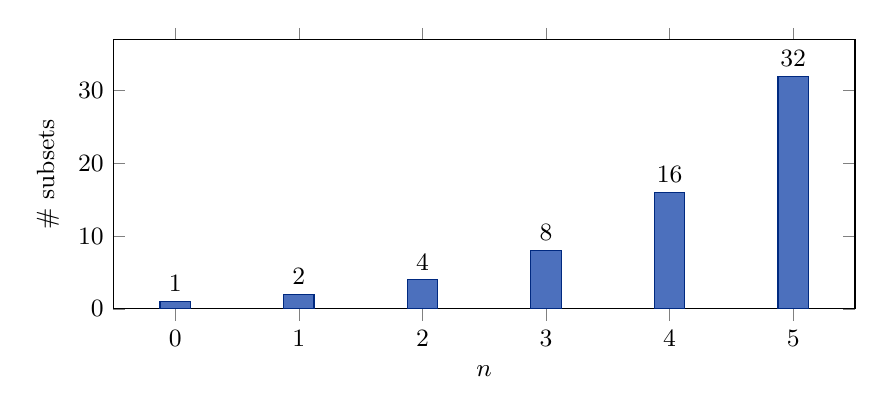
\begin{tikzpicture}
\begin{axis}[
  width=11cm, height=5cm, ybar, bar width=11pt,
  xlabel={$n$}, ylabel={$\#$ subsets}, ymin=0, ymax=37,
  xtick={0,1,2,3,4,5}, nodes near coords, every node near coord/.append style={font=\small},
  tick label style={font=\small}, label style={font=\small}]
\addplot[fill=armBlue!70, draw=armBlue!80!black] coordinates {(0,1)(1,2)(2,4)(3,8)(4,16)(5,32)};
\end{axis}
\end{tikzpicture}
% For 3+ series (e.g. comparing growth rates) use the palette and label series, e.g.:
%   \addplot[armRed,  mark=square*] coordinates {...};
%   \addplot[armBlue, mark=*]       coordinates {...};
%   \addplot[armOrange, very thick, mark=triangle*] coordinates {...};
\end{center}

\begin{methodbox}
\textbf{Transferable technique:} when each part of an object is chosen \emph{independently},
multiply the per-part counts (the product rule). A bijection to bit strings (\textquotedbl{}in/out\textquotedbl{} per element) is the cleanest way to see it.
\end{methodbox}

% --- Reusable TikZ snippet: a "build a bigger object from a smaller one" case split.
% Handy for motivating recurrences / structured counts. Adapt or delete.
\begin{center}

\begin{tikzpicture}[font=\small, >=Stealth,
  blk/.style={draw, rounded corners=2pt, minimum height=8mm, align=center, fill=armBlue!10},
  bit/.style={draw, rounded corners=2pt, minimum height=8mm, minimum width=8mm, fill=armRed!15}]
\node[anchor=east] at (-0.3,0) {add element $x_n$:};
\node[blk, minimum width=4cm] (g) at (2.4,0) {subset of $\{x_1,\dots,x_{n-1}\}$};
\node[bit, right=1.2mm of g] (b) {in / out};
\node[anchor=west] at ($(b.east)+(0.4,0)$) {$\rightarrow$ doubles the count};
\end{tikzpicture}
\end{center}

% ============================================================================
% >>> Add the remaining problems here, each with the same structure:
%     problembox -> ideabox (the WHY) -> Steps -> check -> \answer -> methodbox
%     -> illustration when it genuinely helps.
% ============================================================================

\end{document}
